\documentclass{beamer}
\usetheme{Madrid}

\usepackage{pifont}
\usepackage{enumitem, xcolor}
\usepackage{graphicx}
\usepackage{subcaption}

% default path to images and other assets
\graphicspath{{assets/}}

% disable wrapping
\tolerance=1
\emergencystretch=\maxdimen
\hyphenpenalty=10000
\hbadness=10000

% number figure caption
\setbeamertemplate{caption}[numbered]

% display bib label in references
\setbeamertemplate{bibliography item}{\insertbiblabel}
\setbeamertemplate{bibliography entry title}{}
\setbeamertemplate{bibliography entry location}{}
\setbeamertemplate{bibliography entry note}{}

% props and cons lists
\newlist{propslist}{itemize}{1}
\setlist[propslist]{label=\textcolor[HTML]{3C8031}{\ding{51}}}
\newlist{conslist}{itemize}{1}
\setlist[conslist]{label=\textcolor{red}{\ding{54}}}

% Metadata
% ------------------------
\title[Scientific metrics]{Scientific Metrics}

\author[O. Shkalikov \and M. Zannini \and Q.Qaribiyan]
{Oleh Shkalikov \and Matteo Zannini \and Qader Qaribiyan}

\institute[]{TU Dresden, Computer Science Faculty}

\date{December, 2022}

% ------------------------

\begin{document}

\frame{\titlepage}

\begin{frame}
    \frametitle{Agenda}
    \tableofcontents
\end{frame}

\section{Introduction}

\subsection{Impact factoreesdsd}
\begin{frame}

    \frametitle{Problem}

    \textbf{The original purpose of scientific publishing} was to enable the global sharing of scientific results, ideas, and discussions within the academic society for more effective scientific achievements.\\~\

     \textbf{Influence of a publication is used for :}

\begin{itemize}
   \item allocation of funding resources
   \item industrial and economic growth priorities
   \item  education policies, 
   \item  the hiring of personnel academics
\end{itemize}

\end{frame}
\subsection{Bibliographic Databases}
\begin{frame}
    \begin{figure}[h]
        
\includegraphics[height=0.41\textheight]{s.png}
        \caption{The colors of different sources of attention}
    \end{figure}
\end{frame}
\begin{frame}

    \frametitle{Bibliographic Databases}

    \begin{block}{What is a bibliographic database?}
        bibliographic databases are the main sources of publication metadata and citation metrics
    \end{block}

    A bibliographic database provides an index of journal articles from multiple journals and includes citations, abstracts, and often a link to the full text.\\~\

     \textbf{Frequently used biomedical databases include}
    \begin{itemize}
   \item Web of Science
   \item Scopus 
   \item  Google Scholar 
   \item  The Medline database
   \end{itemize}
\end{frame}
\begin{frame}

    \frametitle{Limitations }
    \textbf{Limitations of bibliographic databases}
    \begin{itemize}
   \item Web of Science
   \item Scopus 
   \item  Google Scholar 
   \item  The Medline database
   \end{itemize}
\end{frame}
\begin{frame}

    \frametitle{Scientific Metrics Types}
     \textbf{Journal-level metrics} are used to determine the impact a journal has on the scientific community\\~\

     \textbf{Article-level metrics} are used to quantify the impact of published articles-how published papers are being discussed and shared.\\~\

    \textbf{Author-level metrics} assess the impact an author makes on the scientific community or field of the study.\\~\

\end{frame}
\begin{frame}

    \frametitle{Problem}

    \textbf{Assessing} the quality and impact of research outputs is necessary \\~\



     \textbf{Every Metric} has its limitations\\~\



    \textbf{No easy way exists} to measure scientific performance\\~\


\end{frame}

\begin{frame}

    \frametitle{Bibliometric Incentive}

    \begin{figure}[h]
        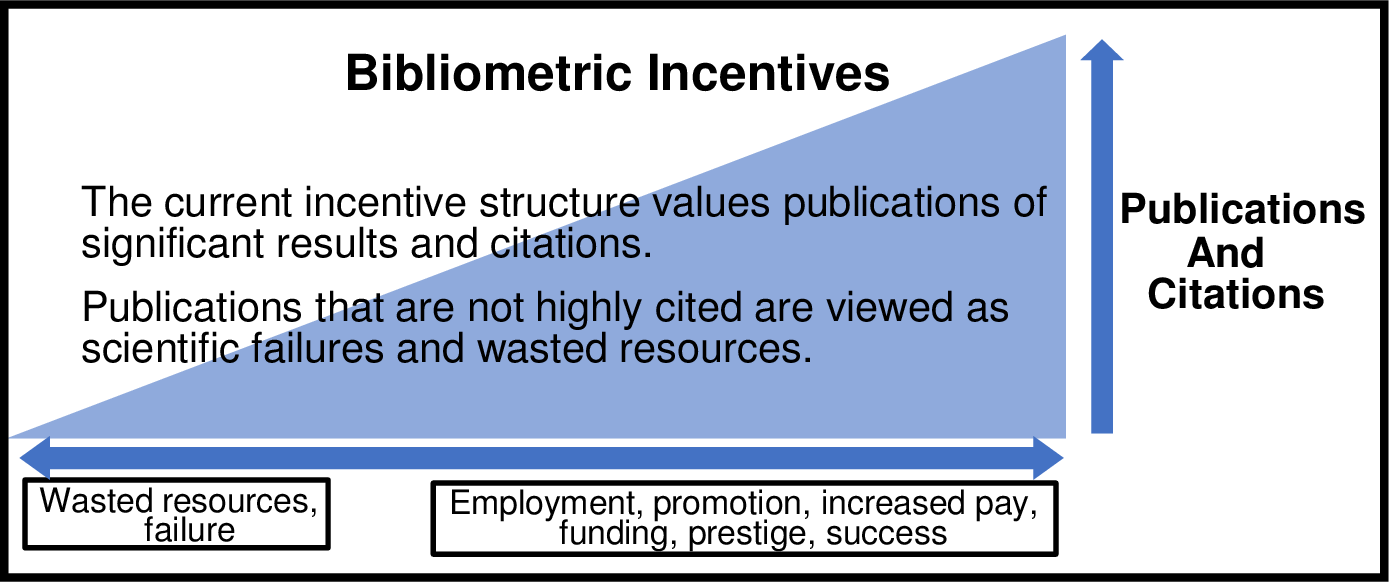
\includegraphics[height=0.5\textheight]{1.png}
        \caption{Bibliometric incentives model. \footnote{https://doi.org/10.1371/journal.pone.0195321.g001}}
    \end{figure}

\end{frame}

\section{Bibliometrics}

% Use section and subsection to add the item to table of contents
\subsection{Impact factor}
\begin{frame}
    \frametitle{Impact factor}

        \begin{block}{What is Impact Factor ?}
        The Impact Factor is the average number of citations received by articles in a journal within a two-year window
    \end{block}
    \begin{align*}
        IF(x) &= \frac{ Citations(x)}{ Publications(x - 2 ) +  Publications(x - 1) }\\
    \end{align*}
    
    \begin{alertblock}{Note}
      Note that 2020 impact factors are reported in 2021; they cannot be calculated until all of the 2020 publications have been processed by the indexing agency.
    \end{alertblock}


\end{frame}
\begin{frame}
    \frametitle{Impact factor limitations}
    \begin{columns}[T]
        \begin{column}{.5\textwidth} \pause
            \centering Advantages
            \begin{propslist}
                \item It gives an idea of the journal’s relative importance and reputation. \pause
            \end{propslist}
        \end{column}
        \begin{column}{.5\textwidth}
            \centering Disadvantages % example how to center one block
            \begin{conslist}
                \item It doesn’t adjust for the distribution of citations \pause
                \item Impact Factors can show significant variation year-on-year.  \pause
                \item Not every journal has an Impact Factor.  \pause
            \end{conslist}
        \end{column}
    \end{columns}
\end{frame}
\begin{frame}
    \frametitle{Altmetric Attention Score}

    \textbf{Altmetric Attention Score} tracks online shares and conversations relating to a piece of published research. \\~\

     It is calculated using data collected around research articles such as mentions on social media, news outlets, blogs, patents, etc.\\~\

    \begin{figure}[h]
        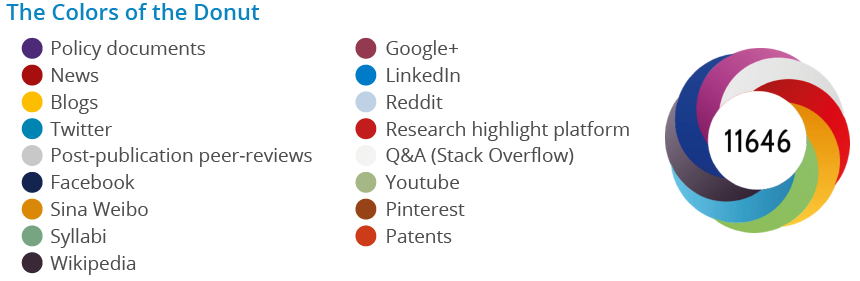
\includegraphics[height=0.41\textheight]{2.png}
        \caption{The colors of different sources of attention}
    \end{figure}
\end{frame}
\begin{frame}
    \frametitle{Advantages to using altmetrics and limitations}
    \begin{columns}[T]
        \begin{column}{.5\textwidth} \pause
            \centering Advantages 
            \begin{propslist}
                \item quicker to accumulate than citation-based metrics  \pause
                \item capture more diverse impacts than citation-based metrics \pause              
                \item Actively engage with comments and conversation around your work \pause
            \end{propslist}
        \end{column}
        \begin{column}{.5\textwidth}
            \centering Disadvantages % example how to center one block
            \begin{conslist}
                \item Altmetrics don’t tell the whole story \pause
                \item People can artificially inflate the altmetrics for their research \pause
                \item Altmetrics are relatively new, more research into their use is needed  \pause
            \end{conslist}
        \end{column}
    \end{columns}
\end{frame}


\begin{frame}[allowframebreaks]
    \frametitle{References}

    \bibliographystyle{apalike}
    \bibliography{references.bib}

\end{frame}

\end{document}